\documentclass[11pt]{article}
\usepackage{lipsum}
\usepackage[margin=2.5cm, includefoot]{geometry}
\usepackage{fancyhdr}
\usepackage{verbatim}
\usepackage{graphicx}
\pagestyle{fancy}
\begin{document}
	\begin{titlepage}
		\begin{center}
			\line(1,0){300}\\
			[0.25in]
			\huge{\bfseries To Create and Compare the Predictive Accuracy of a Genetic Program and an Artificial Neural Network to Predict Company Failure: Final Report}\\
			\line(1,0){300}\\
			[1.5cm]
			
			 \textsc{Carl Saptarshi}\\
			 \textsc{\large  Student Number: 640032165 \\
			 April 2017}
			 
		\end{center}
	\end{titlepage}

\tableofcontents
\thispagestyle{empty}
\cleardoublepage
\setcounter{page}{1}
\section{Background and Introduction }\label{sec:intro}
Due to the dynamic and volatile economy that we live in, the number of companies filing for bankruptcy are on the rise, especially during times of economic uncertainty, for example, during a period of recession.\\
In turn, being able to predict the likelihood of a company failing and filing for bankruptcy is very important and has been a focal point of issue in accounting research and analysis over the past thirty years. 

\subsection{Background into Bankruptcy}
\subsubsection{What is Bankruptcy? }\label{sec:bankdef}
When a company (the \textit{debtor}) takes out a loan or borrows money from somewhere else such as a financial institution like a bank (the \textit{creditor}) , it is up to the debtor to ensure that the creditor is repaid the full amount that was borrowed subject to the creditors terms and conditions.


If the debtor starts to fall behind on their payments to the point that they are unable to repay their debts or unable to keep up with the incremental loan repayments, the debtor may file for a Chapter 7 bankruptcy in which the court will appoint a trustee to shut down the company and liquidate their assets, for example, by selling machinery, land and company shares to recover some money which they the trustee can give back to the creditor to clear the company's debt. If the company is still unable to pay back the debt even after this, then they will file for bankruptcy and the company will be terminated. Since the 1960's, as economies have grown, especially in the western world, this problem has been recognised on grander scale in more economically developed countries.

\subsubsection{Who does it affect?}
Bankruptcy does not just affect those that are employed within that company; it also affects third party members such as shareholders, investors, suppliers, and company clients . CF has been a critical point of focus, especially in the field of financial analysis and for stakeholders who are interested in the performance of the company. Since the 1960's, empirical risk assessment models have been developed which have been used to predict CF. Using current and previous financial data of a company, the likelihood of CF can be predicted for 'n' number of years ahead. This in turn means that loan companies, such as banks, can use this information to determine whether loans should be granted to other firms, knowing the likelihood of a company defaulting or not. This has helped to give banks competitive advantages, as they become aware of how likely a company will be to default, and therefore is able to predict customer behaviour in times of difficulty.\\
Looking at reports from the American Bankruptcy Institute showed that in the year 2000, 35,742 companies filed for bankruptcy, 43,546 companies in 2008 and 60,837 by 2009, at the peak of the recession. By 2012 this fell to 40,075 and 24,114 by 2016. These statistics clearly indicate the volatility and uncertainty in the economy as it changes, which is part of what makes CF prediction incredibly important, especially for those involved with the company at hand.

\subsection{Algorithms for Company Failure prediction}
Since the aim of the project to classify whether a company is likely to fail or not, this can be called a binary classification problem which will take in a series of inputs and return a classification which determines whether a company is financially distressed or not. On top of this, a company likely to suffer from financial distress will have certain characteristics associated with them, similarly this would occur for companies not facing this problem. This means that the data should be linearly separable when classifying the data, making this a linear binary classification problem. \\
There have been several techniques that have been used to predict CF, some of which will be introduced here.  

\textbf{Individual Ratio Selection (IRS)} -In the 1960's, Beaver introduced IRS. This process involved selecting thirty financial variables, converting these to ratios. Based on a certain threshold for each variable, this would determine if a company is likely to fail or not.

\textbf{Multivariate Discriminant Analysis (MDA)} - Altman created this technique in the 1960's, which takes uses a discriminant function to score a company. This function uses five financially weighted ratios and based on the overall discriminant score, the company can be classified. 

\textbf{Genetic Programming (GP)} - GP's are inspired by Darwin?s Theory of Evolution, used for prediction and classification. A population of functions is created and fitter individuals in the population are more likely to survive and produce offspring that are even more suited to the environment. The aim is to create an optimal function which can give the most accurate prediction in terms of classification accuracy. 

\textbf{Artificial Neural Networks (ANN)} - This technique is inspired by the interconnectivity of the brain and applies this to prediction and classification. ANN's are made of an input layer, hidden layers and the output layer which outputs the classification based on the input. The network uses the weights on the synapses of the nodes that connect one node to the next, which are tweaked to allow the network to learn and give a more accurate classification for unknown datum. 

\textbf{Supervised Learning} - GP's and ANN's fall under the umbrella of Machine Learning (ML). ML is a form of Artificial Intelligence (AI) that allows a computer program to learn without the use of explicit programming. This means whilst the program is running, it will start to form patterns based on the data that is fed in, and adapt the program appropriately to try to produce the best results until a termination criteria is met.
In supervised learning, the output after each iteration of each algorithm is compared against the already known desired output. This can then be used for comparison to check whether or not the programs have correctly classified a company financially distressed or not. For every iteration, the program will start to learn, so the accuracy of the classifications will start to increase over time. Eventually, when an unknown set of data is inputted into the programs, the program will be able to correctly produce an output to declare if the company in question will likely to fail or not along with a percentage of certainty.\\ 



\subsection{Motivations For this Project}
\newpage
\section{Summary of literature review and specification}\label{sec:spec}
\subsection{Literature Review}
All the techniques mentioned in section 1.2 have been used extensively in the classification and prediction of problems. Altman and Ohlson, who are the pioneers of CF prediction since the 1960's used selected financial variables from multiple companies bank statements to predict CF. These variables (\textit{key performance indicators} (KPI's)) were used as they believed were important factors that indicated whether a company was financially distressed. To make companies more comparable, both techniques involved converting the KPI's into ratios as a method of standardising the data. Due to the success of both of their methods, newer techniques proposed are based around their financial ratios and use the prediction accuracy for both methods as benchmarks to compare their new proposed work against techniques already in use. \\

Overall, Altman's technique was superior to Beaver's method, but only if the KPI's were jointly distributed according to a multivariate normal distribution. Otherwise, it was prone to errors. However, the MDA technique was favoured as it could use multivariate data at once to get an overall prediction rather than taking each ratio and scoring that to give predictions. \\
Wilson and Lensburg took modern approaches by implementing ANN's and GP's to this classification problem. Both techniques can handle noisy data that is not normally distributed better than Altman's MDA, showing that both ANN's and GP's have potential to be more accurate than IRS and MDA. 

ANN's tend to perform very well in terms of efficiency and accuracy. Wilson used an ANN approach with a 5 10 2 structure. To improve accuracy, the Monte-Carlo technique was used to give a better representation of predicative accuracy. Overall, they achieved a 97.5\% accuracy on their testing dataset, making this much more accurate than MDA and IRS. \\
ANN's suffer from being unable to produce a readable function to indicate how it came to the solution, other than viewing the synaptic weights. Another issue faced  is that since a function is unable to be produced, the ANN is unable to tell us what influence each KPI has when predicting CF.\\
GP's can overcome some of the problems of an ANN as they are able to produce a user readable function. It is possible to see what kind of influence each KPI has relative to each other. Lee used a decision tree (DT) method to predict CF. Lee used eight different KPI's when approaching this problem. Using this GP method, the testing accuracy of 92.91\%. Rostamy used a similar approach to Lee, using five different KPI's. After training the GP, it could correctly predict if a company would fail 90\% of the time, which was like MDA, however more flexibile in terms of what type of data it could accept. \\
GP's may work slower as they explore a large search space and may be restricted to certain limitations e.g. a maximum tree depth. For each crossover and mutation, the depth of tree may increase. This can increase the computation time rapidly. When designing and implementing the GP, these factors will typically be accounted for as seen in Etemadi's et al paper. \\
\\
Through the research completed, many papers used Altman's KPI's as their inputs. However, as Altman suggested, these ratios may not necessarily be the most optimal, but these still provided the best alternative discriminant function to work with at the time. Since then economies have changed significantly, these ratios may not necessarily be the best to use to predict CF, but may still be significant enough to give an accurate prediction. As seen by Back, Rostamy and Lee, other ratios have been used to predict CF, and achieved similar results to MDA, which could potentially be more significant now. Wilson used Altman's KPI's and achieved the 97.5\% accuracy, with far fewer ratios relative to Back and Lee, which must be taken into consideration.

\subsection{Project Specification}
After careful consideration of the researched techniques, I will be predicting CF using ANN's and GP's due to their strong accuracy rates and ability to handle noisy data. though they do have drawbacks, I will aim to minimise these through the project specification and implementation.\\
\\
A dataset of 134 different Small-Medium Enterprises (SME?s) were collected, using between three to five years? worth of data for each, giving a total of approximately 700 data records. The decision to use SME?s was to have more consistent, comparable data, as shown by Altman.The spreadsheet consists of financial statement names and variables which can be used for the programs that will be made. To begin with, I will use Altman's KPI's as these have proven to be successful even today. 
The data provided also shows whether or not a company has failed not failed during a certain time period. Since there are KPI's which will be used, and a clear binary output (0 or 1) which is known and will be used, this type of ML is known as a supervised learning task. \\

Two programs will be created for this project. Firstly, a feed forward ANN with back propagation and secondly a regression tree GP will be created. The reasons that I have chosen to use these are due to the research that I have undertaken, ANN?s have been known to produce very accurate results in an efficient time manner. The reason that GP is a valid technique to use for this task is that GP?s can be used in prediction, but also they are able to create a function that will directly map the input to the output in order to produce the given result. \\
For the ANN, I will use a library - \textit{sklearn}, a module in the Python programming language,  as this library consists of optimised mathematical functions which will enable the creation of the ANN to be much easier due to possible time constraints, and because this will used as a benchmark to test against the GP. Although sklearn does provide support for regression trees in Python, I will make it from scratch, as this will provide me with more flexibility to manipulate the functions more easily towards the problem at hand. 
Once The GP and ANN have been created, run, and the results tabulated and graphed, I will then be able to test each one independently and against each other. They will also be compared to Altman's benchmarks to compare the predictive accuracies from the two programs I will be making. \\\\
The task is also known as a binary classification problem. This means that the output of each of the programs determine whether a company can be classified as likely to fail or will not fail. To represent this classification, the value of 0 will represent a non-distressed company, and a 1 will represent a financially distressed company.
Since this representation will be a number, in order to break this down further, the actual floating point value of the output (which will be between 0 and 1) will be used  to represent the likelihood of failure as a probability. For example, if the value was 0.618, it could be said that the company has a probability of 0.312 of staying afloat for the forthcoming year. Whereas if the value was 0.111 then the company has a 0.899 probability of staying afloat for the forthcoming year. Here, a clear differentiation can be made between two companies, one which is more likely to fail than the other.


\newpage
\section{Design}
\begin{figure}[h]
\centering
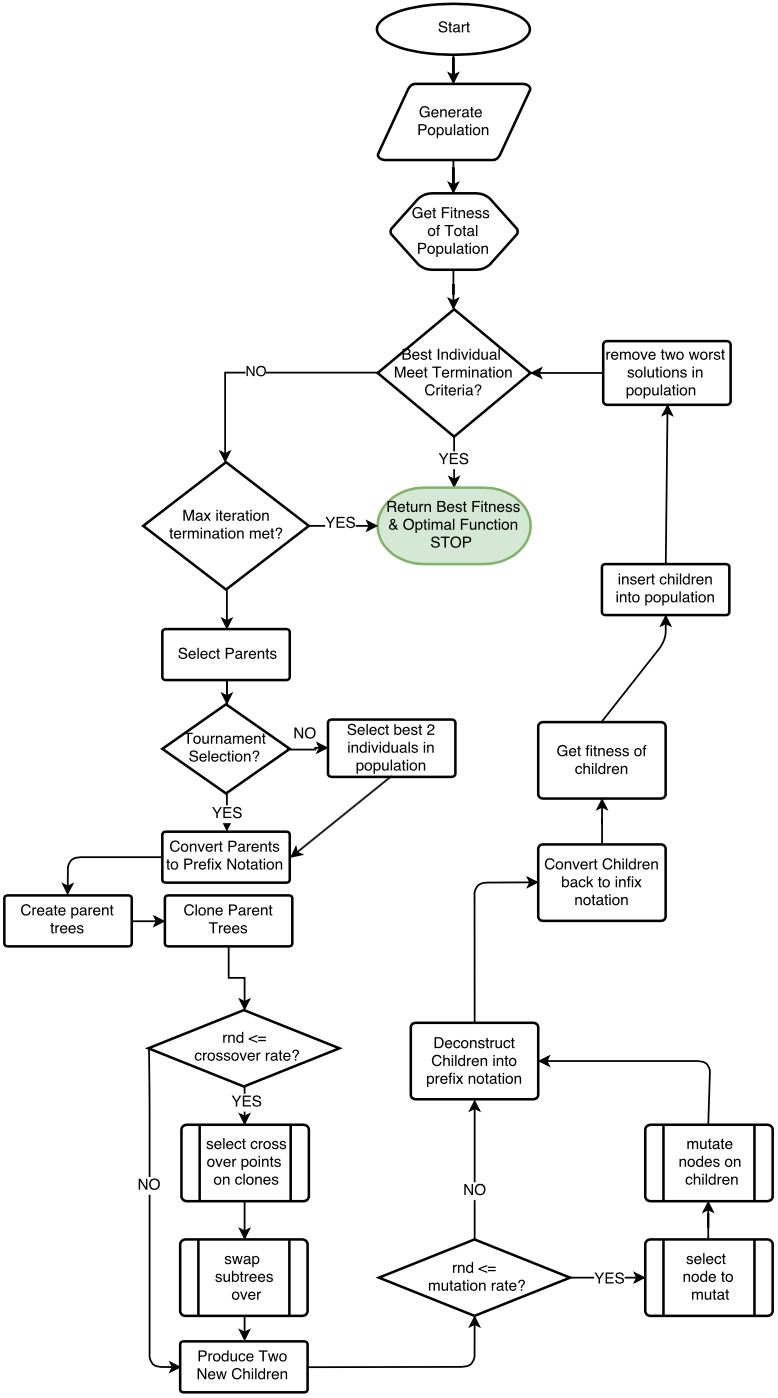
\includegraphics[scale = .67]{flown}
\end{figure}
hellooo world hellooo world hellooo world hellooo world hellooo world hellooo world hellooo world hellooo world hellooo world hellooo world hellooo world hellooo world hellooo world hellooo world hellooo world hellooo world hellooo world hellooo world hellooo world hellooo world hellooo world hellooo world hellooo world hellooo world hellooo world hellooo world hellooo world hellooo world 


\newpage
\section{Development}

\newpage
\section{Testing}

\newpage
\section{Description of the final product}

\newpage
\section{Evaluation of the final product}

\newpage
\section{Critical assessment of the project }

\newpage
\section{Conclusion}


\newpage
\section{Antohny page}



\end{document}


